\documentclass{article}

\usepackage{graphicx}
\begin{document}
\setlength\parindent{0pt}

\textbf{Important Notes}\\
Video was done 8 months ago\\
Mariusz was hired by the company to promoted STOCK

\section{ADURO}

\begin{itemize}
  \item Ofer Vicus (CEO)
  \item Public since 2021
  \item They have been doing R\&D for 10 years until they recently went public
  \item ADURO not making revenue (at first Mariusz as not interested because of it)

  \item ADURO claims to solve a problem that is says to have a 2025 deadline,
    even though there are no revenues, the idea to solve this problem transforms
    this to a more attractive investment

  \item What is the problem? Plastic 
    \begin{enumerate}
      \item Plastic is becoming one of the most problematic component for the
        environment
      \item By 2025, there is a deadline for the big plastic producers to reduce
        the plastic consumption and recycling 
    \end{enumerate}
  \item ADURO, has created a new approach to manage plastic consumption. 
    uses the 80\% that nobody else can process in order to recycle it, around 20\% of the
    plastic is easy to manage and recycle, but there are no other competitors
    that can manage that 80\% of plastic. Is a technology based on water.
  \item Many big players (as he called them) are already interested in ADURO,
    and each of the interested parties can return millions of dollars each
\end{itemize}

\subsection{Proposed Business Model}
\begin{itemize}
  \item Licensing model
    Customer puts out their own factory or recycling facility and ADURO charges a licensing fee, (highest in returns)
  \item Own Producing Model
    ADURO setup their own recycling facility 
\end{itemize}


\subsection{Margin of Safety (How much money can I loose?)}
Things that provides Mariusz margin of safety
\begin{itemize}
  \item Insiders (of the company) own 48\% of the company, so there is a
    pressure to succeed
  \item The patents are owned by them
  \item Cost of patents
  \item Scientists backup the technology used by ADURO

\end{itemize}

\subsection{Market Today and Forecast}
\textbf{April 05$^{th}$} 0.95 CAD\\
  He states that in around 5 years the return could be exponential
  
\begin{figure}[h]

\begin{center}
  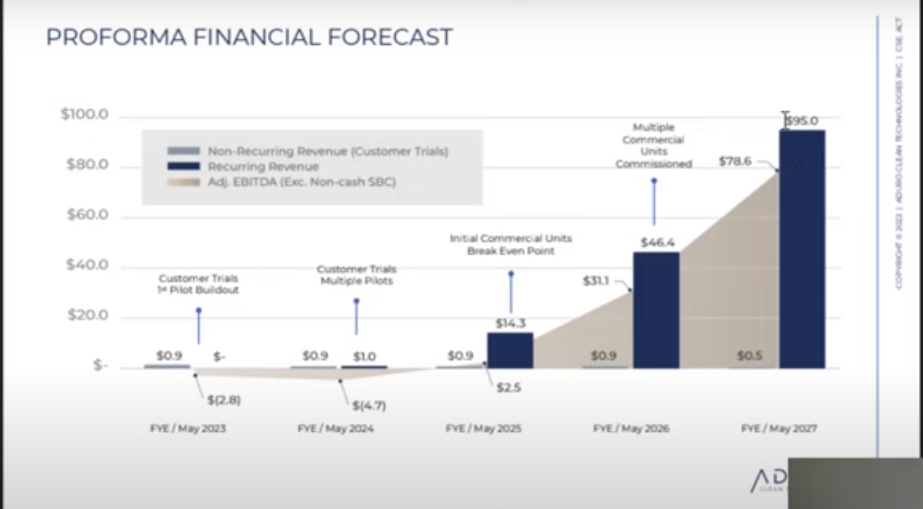
\includegraphics[scale=0.3]{figures/forecast.png}
\end{center}
\caption{Forecast presented by ADURO}
\label{fig:forecast}
\end{figure}

\subsection{Scientific Ideas behind the Company}

Next Generation Chemical Decostruction Technology
\begin{enumerate}
  \item Converting waste plastics to the manufacturing of new plastics (recycling)
\end{enumerate}


\subsection{Patents}
The CEO of the company when asked by Mariusz how much money does the company
(saying company as their procedures and patents) cost right now. He answered
that around 20 to 50 million dollars. Later he mentions that he would sell it by
no less than 200 million.
\begin{itemize}
  \item 
\end{itemize}

\end{document}



